\chapter{Anti-de Sitter space in dimension (2+1)}
We will now restrict our attention to dimension three Anti-de Sitter geometry, as it will be the specific model geometry of the manifolds of our next interest. In this chapter we will highlight the structure of Lie group that $\A^{2,1}$ has in this specific dimension and we will study its geometry using tools of Lie group theory. Most of the results are just a particular case of the theory developed in the previous chapter, but the Lie structure permits to give a more explicit description of the geometry of the phenomena we are interested in.\\

\section{The {PSL}$(2,\R)$ model} 
The fundamental observation is the existence of a special model in dimension three which endows Anti-de Sitter space with a Lie group structure. To construct such a model we observe that $q=-$det is a quadratic form with signature (2,2) over the real vector space $\mathcal{M}(2,\R)$ (the signature is evident when we consider the basis consisting of elementary matrices). The associated bilinear form is expressed by the formula:
\begin{equation}\label{quadratic}
    \langle A,B\rangle=-\frac{1}{2}\text{tr}(A\cdot\text{adj}(B))
\end{equation}
for $A,B\in\mathcal{M}(2,\R)$, where adj denotes the adjugate matrix, namely: 
\[
\text{adj}\Big(\begin{bmatrix}
    a & b \\
    c & d
\end{bmatrix}\Big) = \begin{bmatrix}
    d & -b \\
    -c & a
\end{bmatrix}
\]

hence, via Sylvester's theorem, there is an identification between $(\mathcal{M}(2,\R),q)$ and $(\R^{2,2}, q_{2,2}),$ unique up to composition by elements in $O(2,2)$. Under this isomorphism $\H^{2,1}$ is identified with the Lie group $\text{SL}(2,\R).$\\
Let us observe that $\text{SL}(2,\R)\times \text{SL}(2,\R)$ acts linearly on $\mathcal{M}(2,\R)$ by left and right multiplication:
$$(A,B)\cdot X=AXB^{-1}.$$

As a direct consequence of the Binet formula, the action preserves the quadratic form $q$    and thus induces a representation: 

\[ \rho:\text{SL}(2,\R)\times \text{SL}(2,\R)\to O(\mathcal{M}(2,\R),q). \]

Since the center of $\text{SL}(2,\R)$ is $\{\pm \text{Id}\},$ the kernel of $\rho$ is $K=\{(\text{Id},\text{Id}),(-\text{Id},-\text{Id})\},$ and by a dimensional argument (and connectedness of $\text{SL}(2,\R)$) it turns out that the image of the representation is the connected component of the identity: 
\[
    \text{Isom}_0(\H^{2,1})=\text{SO}_0(\mathcal{M}(2,\R),q)\simeq (\text{SL}(2,\R)\times \text{SL}(2,\R))/K
\]
    
Using this model, one has a natural identification between $\A^{2,1}$ and the Lie group $\PSL$, in such a way that: 
\begin{equation}\label{isomiso}
    \text{Isom}_0(\A^{2,1})\simeq \PSL\times\PSL
\end{equation}
    
acting by left and right multiplication on $\PSL$.\\ We are mostly interested in orientation-preserving and time-preserving notions that do not depend on a chosen orientation, nevertheless we will fix here an orientation and a time-orientation of $\A^{2,1}\simeq\PSL.$ As we are dealing with a Lie group it is sufficient to define an orientation of the Lie algebra, namely the tangent at the identity Id. We declare as (positive) oriented basis of $\mathfrak{sl}(2,\R):$ 
\begin{equation}\label{tangent}
V=\begin{pmatrix}
  0 & 1 \\ 1 & 0
\end{pmatrix}\;\;
W=\begin{pmatrix}
1 & 0 \\ 0 & -1
\end{pmatrix}
\;\;
U=\begin{pmatrix}
0 & -1 \\ 1 & 0
\end{pmatrix}
\end{equation}

The first two vectors $V,W$ are spacelike, while $U$ is timelike. $U$ is the tangent vector to the one-parameter group of elliptic isometries of $\H^2$ fixing $i\in\H^2$, parametrized by the angle of clockwise rotations; $V,W$ are vectors tangent to the one-parameter groups of loxodromic isometries fixing the geodesic with endpoints $(-1,1)$ and $(0,\infty)$ respectively. Time-orientation can also be inherited by the Lie algebra, we declare that $U$ is a future-pointing timelike vector. \\

The stabilizer of the identity in Isom$_0(\A^{2,1})$ is the diagonal subgroup $\Delta<\PSL\times\PSL$. Under the obvious identification of $\PSL$ and $\Delta,$ the action of the identity stabilizer on the Lie algebra $\mathfrak{sl}(2,\R)=T_{\text{Id}}\PSL$ is the adjoint action of $\PSL$. A direct consequence of this construction is the bi-invariance of the quadratic form $q$. Indeed, denoting by $q_{\text{Id}}$ the restriction of $q$ to $T_{\text{Id}}\text{SL}(2,\R)$, a direct computation shows that $q_\text{Id}$ equals $(1/8)\kappa$ where $\kappa(X,Y)=4tr(XY)$ is the Killing form of $\mathfrak{sl}(2, \R)$.

\begin{observation}\label{311}
    The Lie algebra $\mathfrak{sl}(2,\R)$ equipped with the quadratic form $q_{\text{Id}}$ is then a copy of the 3-dimensional Minkowski space, hence the adjoint action yields a representation 
    \[
        \PSL\to O(\mathfrak{sl}(2,\R),q_{\text{Id}})
    \]

which in turn induces the well-known isomorphism: 
\[
    \text{SO}_0(2,1)\simeq\text{SO}_0(\mathfrak{sl}(2,\R), q_\text{Id})\simeq \PSL,
\] which is nothing but the restriction of the isomorphism of Equation \ref{isomiso} to the stabilizer of the identity in the left-hand side $(\text{Isom}(\A^{2,1})),$ and to the diagonal subgroup $\Delta$ in the right-hand side $(\PSL\times\PSL).$
\end{observation}

\section{The boundary of $\PSL$} 
From the aforementioned identification we obtain a new one between $\partial\A^{2,1}$ with the boundary of $\PSL$, inside $\text{P}(\mathcal{M}(2,\R))$ as the projectivization of the cone of rank 1 matrices. Therefore from now on we shall consider 
\[
    \partial\A^{2,1}=\{[X]\in\text{P}(\mathcal{M}(2,\R))|\;\text{rank}(X)=1\}.
\]
We endow $\overline{\A^{2,1}}\coloneqq \A^{2,1}\cup\partial\A^{2,1}$ with the topology induced by seeing both as subsets of the real projective space $\text{P}(\mathcal{M}(2,\R)).$ We want to observe that we have the following homeomorphism: 
\begin{align*}\label{delta}
    \delta:\partial\A^{2,1}&\rightarrow\R\text{P}^1\times\R\text{P}^1\\
    [X]&\mapsto (\text{Im}(X),\text{Ker}(X))
\end{align*}


where we are considering $\R\text{P}^1$ as the space of one-dimensional subspaces of $\R^2$. Since we have that $\text{Im}(AXB^{-1})=A\cdot\text{Im}(X)$ and $\text{Ker} (AXB^{-1})=B\cdot\text{Ker}(X),$ the map $\delta$ is equivariant with respect to the action of $\PSL\times\PSL,$ acting on $\partial\A^{2,1}$ as the natural extension of the group of isometries of $\A^{2,1}$ and on $\R\text{P}^1\times\R\text{P}^1$ by the obvious product action.\\
In this setting our choice of a time-orientation \textit{can be modified} according to the following Lemma:
\begin{lemma}\label{invertime}
    The inversion map $\iota[X]=[X]^{-1}$ is a time-reversing isometry of $\A^{2,1}$ which induces the homeomorphism $(x,y)\to(y,x)$ on the boundary $\partial\A^{2,1}.$
\end{lemma}
\begin{proof}
    It follows from definition that $\iota$ is equivariant with respect to the isomorphism of $\PSL\times\PSL$ which switches left and right factors, more explicitly we have that for every $A,B\in\PSL$ the following holds: $\iota[(A,B)X]=(B,A)\cdot[\iota X]=BX^{-1}A^{-1}$. As $\text{d}_\text{Id}\iota=-\text{Id}$ is a linear isometry, $\iota$ is an isometry, the differential being minus the identity also shows that it revers time-orientation. \\ 
    The second part of the statement can be checked via the following. For a $2\times2$ matrix the Cayley-Hamilton theorem implies the equality $(\det X)X^{-1}=(\text{tr}X)\text{Id}-X,$ so that projectively we have $[X^{-1}]=[\text{tr}X\text{Id}-X].$ Hence $\iota$ extends to the transformation $[X]\to[\text{tr}X\text{Id}-X]$ on $\partial\A^{2,1}.$ Now if $X$ is a rank $1$ matrix, it is traceless if and only if $X^2=0$, hence $\text{Ker}(X)=\text{Im}(X).$ If $\text{tr}(X)\neq 0$, then $X$ is diagonalizable with eigenvalues $0$ and $\text{tr}(X)$. Moreover $\text{Ker}(X)$ and $\text{Im}(X)$ are the corresponding eigenspaces. It follows then that $\text{Ker}(\text{tr}X\text{Id}-X)=\text{Im}(X)$ and $\text{Im}(\text{tr}X\text{Id}-X)=\text{Ker}X$ 
\end{proof}


Consider the hyperbolic model of the upper half-plane $\H^2.$ $\R\text{P}^1$ corresponds to the boundary at infinity $\partial\H^2$ via the identification mapping the line spanned by $(a,b)$ to $\frac{a}{b}$ and $\PSL$ is identified to $\text{Isom}_0(\H^2$). From this perspective we can consider $\partial\A^{2,1}$ as $\partial\H^2\times\partial\H^2$. We can then interpret the convergence to $\partial\A^{2,1}$ in this setting:

\begin{lemma}\label{convergenza}
    A sequence $[X_n]\in\A^{2,1}$ converges to $(x,y)\in\partial\A^{2,1}\simeq\T$ if and only if for every $p\in\H^2,$ $X_n(p)\to x$ and $X_n^{-1}(p)\to y.$ 
\end{lemma}
\begin{proof}
    Since $\PSL$ acts on $\H^2$ via isometries, if the conditions holds for some $p$ then it holds for all $q\in\H^2$, as the distance from $p$ to any other point $q$ is bounded. Without loss of generality we can assume $p=i$ in the upper half-plane. Assuming $[X_n]=\begin{bmatrix}
        a_n & b_n \\
        c_n & d_n
    \end{bmatrix}$ converges projectively to a rank 1 matrix means that there exists a sequence of real numbers $\lambda_n\to 0$ such that $\lambda_n X_n\to X$. As the limit matrix has rank one at least one of the successions of coefficient (when multiplied by $\lambda_n$) does not converge to zero. We can assume that $\lambda_n a_n\to a$ does not converge to 0, the other cases are all analogous. The assumption of  $a\neq 0$ and rank$(X)=1$, leave us with the following possibilities for $X$:
    \begin{itemize}
        \item Assume $\lambda_{n}c_n\to 0$ and $\lambda_n d_n\to0$, then we have that $[X_n]$ converges to a $[X]$ of the form: $$\begin{bmatrix}
            a & b \\
            0 & 0\end{bmatrix},\; X(i)=\lim_{n\to\infty} \lambda_n\frac{a_n i+b_n }{c_n i+d_n}=\frac{a}{0}$$

        \item If $b=0$ and $d=0$, then $[X_n]$ converges to $[X]$ with $$X=\begin{bmatrix}
            a & 0 \\
            c & 0 \end{bmatrix},\; X(i)=\lim_{n\to\infty} \lambda_n\frac{a_n i+b_n }{c_n i+d_n}=\frac{a}{c}$$
        \item If $b,c \neq 0$ it follows from the rank one condition that $d=bc$, then $[X_n]$ converges to $[X]$ with $$X=\begin{bmatrix}
            a & b \\
            c & \frac{bc}{a} \end{bmatrix},\; X(i)=\lim_{n\to\infty}\frac{a_ni+b_n}{c_{n}i+d_n }=\frac{a^{2}i+ab}{aci+bc}=\frac{a(ai+b)}{c(ai+b)}=\frac{a}{c}.$$
    \end{itemize}
    All the (finite) case left are similar.
    % The convergence of $X_n^{-1}(p)\to y$ is just a straightforward application of Lemma \ref{invertime} and an analogous argument to the one given for $X_n(p)$.
\end{proof} 

In dimension three, $\partial\A^{2,1}$ is a double ruled quadric, which in an affine chart looks like \textcolor{red}{inserire cono}. We shall describe such rulings in a more geometric way. Given any $(x_0,y_0)\in\partial\A^{2,1}$, the set
\begin{equation}\label{ruling}
        \lambda_{y_0}\coloneqq\{(x,y_0)|x\in\R\text{P}^1\}
\end{equation}

describes a projective line in $\R\text{P}^3$ which is contained in $\partial\A^{2,1}$, hence lightlike for the conformal Lorentzian structure of $\partial\A^{2,1},$ as seen in Remark \ref{222}. In fact $\lambda_{y_0}$ is the orbit of $(x_0,y_0)$ by the action of $\PSL\times\{\text{Id}\},$ or by the (now free) action of $\text{PSO}(2,\R)\times\{\text{Id}\}.$ Here $\text{PSO}(2,\R)$ corresponds to a 1-parameter elliptic subgroup in $\PSL$. In short: 
\[
    \lambda_{y_0}=\PSL\cdot(x_0,y_0)=\text{PSO}(2,\R)\cdot(x_0,y_0).
\]

We refer to $\lambda_{y_0}$ as the \textit{left ruling} through $(x_0,y_0)$, and similarly the \textit{right ruling} is the set:
\[
    \mu_{x_0}\coloneqq\{(x_0,y)|y\in\R\text{P}^1\}.
\]
We can express the conformal Lorentzian structure of $\partial\A^{2,1}$ with the rulings as shown in Figure \ref{baleani}. The action of $\text{PSO}(2,\R)\times\{\text{Id}\}$ on $\A^{2,1}$ yields a flow on $\A^{2,1}$ generated by a right-invariant vector field, which at Id is the \textit{positive } tangent vector of $\text{PSO}(2,\R).$ So orbits are all timelike and \textit{future directed}. In similar fashion the action of $\{\text{Id}\}\times\text{PSO}(2,\R)$ yields a flow generated by a left-invariant vector field, which at Id is the \textit{negative} tangent vector at $\text{PSO}(2,\R)$, and its orbits are all timelike and \textit{past directed}. 


\begin{figure}
    \centering
    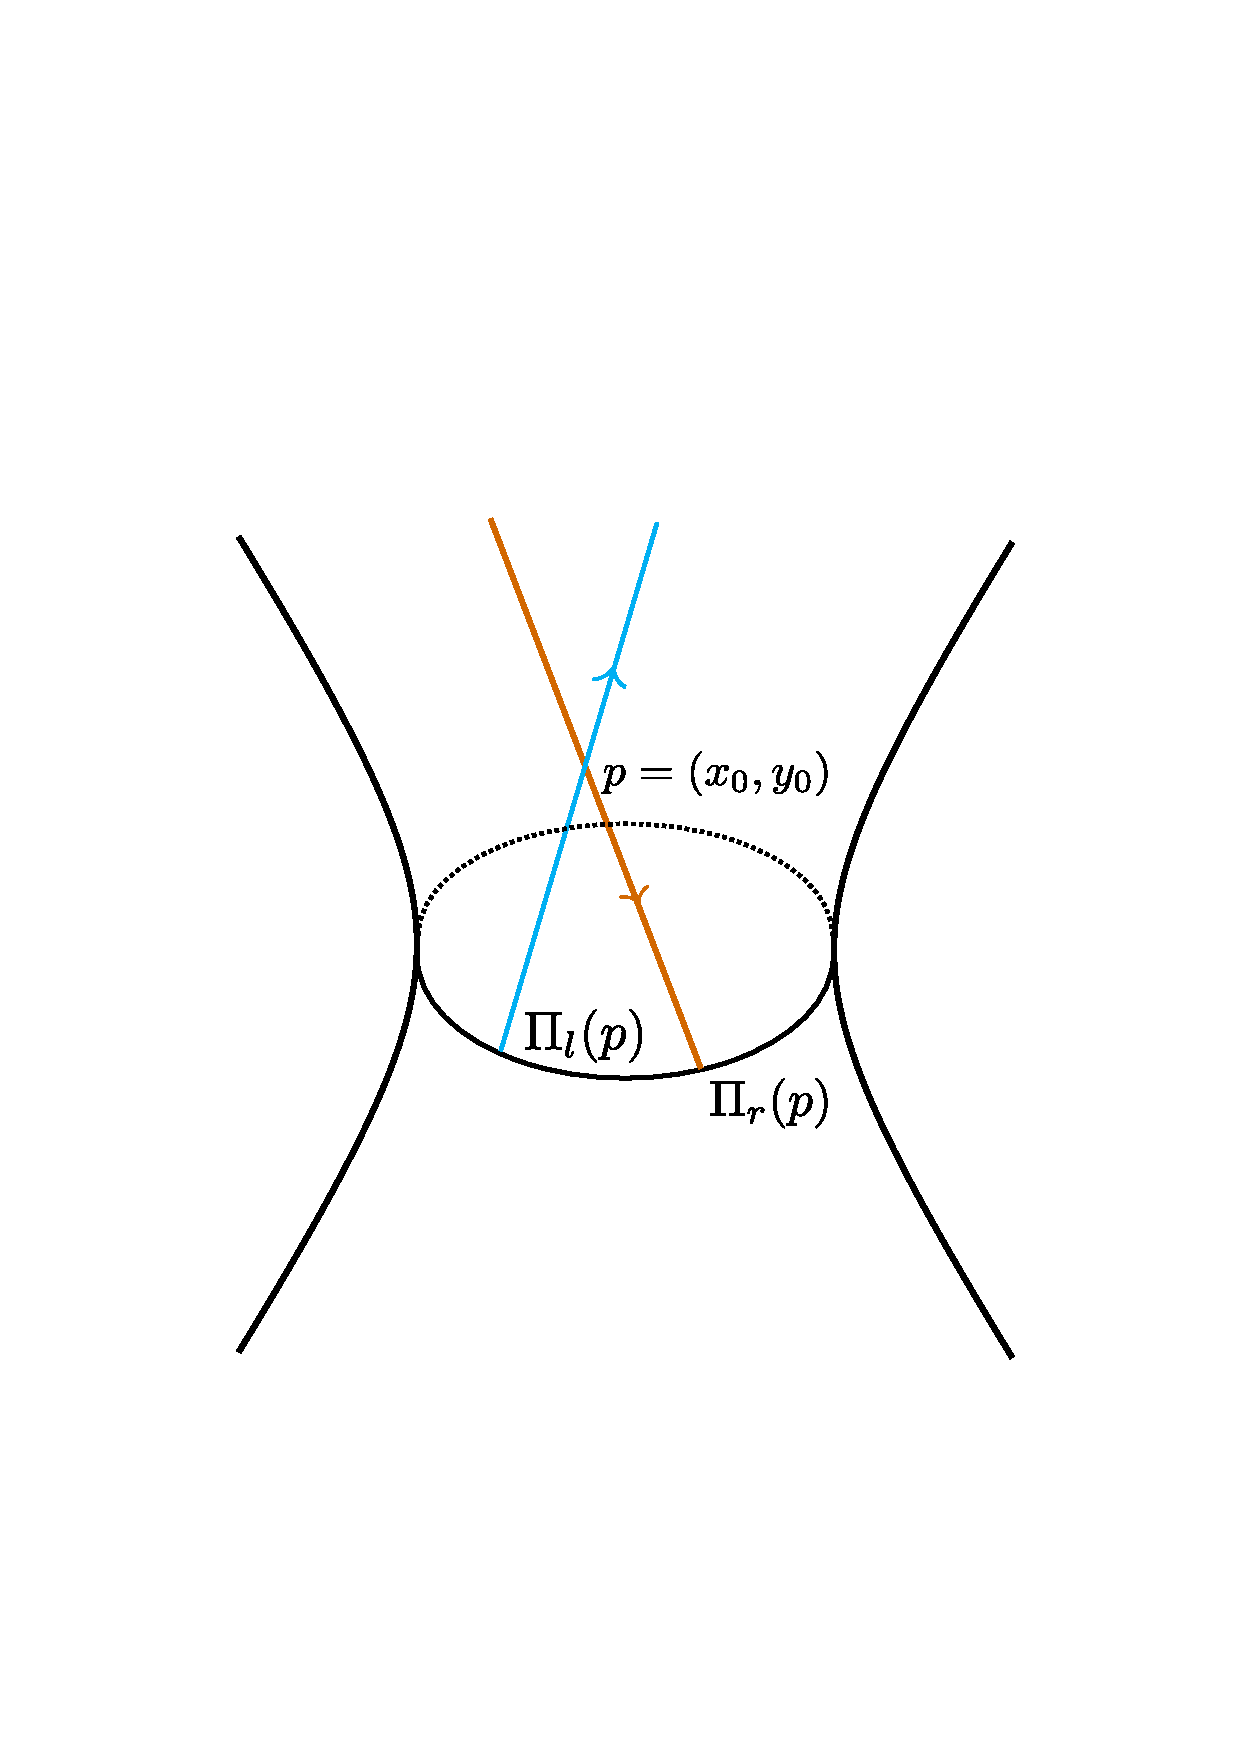
\includegraphics[width=0.7\textwidth]{baleaniperbolato.pdf}
    \caption{Left and right projection from a point $p\in\partial\A^{2,1}$ to the
    plane $P=\{x_3=0\}.$ The rulings induce a time-orientation on the boundary.}
    \label{baleani}
\end{figure}


\begin{proposition}
    Let $\pi_l,\pi_r:\S\times\S\to\S$ be the canonical projection and $d\theta$ be the angular form on $\S\simeq\partial\H^2$. Then the symmetric product $\pi_l^*(d\theta)\pi_r^*(d\theta)$ is in the conformal class of $\partial\A^{2,1}$.
\end{proposition}  
\begin{proof}
 Since we already know that the left and right rulings are lightlike for the conformal class of $\partial\A^{2,1}$, it only remains to check the sign of time orientation. We observe that $\lambda_{y_0}$ is the orbit of the action of $\text{PSO}(2,\R)\times\{\text{Id}\}$, while $\mu_{x_0}$ is the orbit of the action of $\{\text{Id}\}\times\text{PSO}(2,\R),$ the induced orientation agrees with the one given by the pullback of the metrics. 
\end{proof}

\noindent It follows, from the conformal structure that $\partial\A^{2,1}$ inherited from the rulings, that a $C^1$ curve in $\partial\A^{2,1}$ is spacelike when it is locally the graph of an orientation-preserving function (the product of the pullbacks is different from zero and we can use the implicit function theorem), and timelike when it is locally the graph of an orientation-reversing function. Given two intervals $I_1,I_2$ in $\partial\H^2$ and assuming that $\theta_1,\theta_2$ are angle determination over the two intervals, the future $I^+_{I_1\times I_2}(p_0,q_0)$ of a point $(p_0,q_0)$ in $I_1\times I_2$ is the region made up of points $(p,q)$ where $\theta_1(p)-\theta_2(p_0)>0$ and $\theta_2(q)-\theta_2(q_0)<0$. The past is determined by reversing both inequalities. In conclusion: 
\begin{equation}\label{angular}
    I^+_{I_1\times I_2}(p_0,q_0)\cup I^-_{I_1\times I_2}(p_0,q_0)=\{(p,q)\in I_1\times I_2\;|\;(\theta_1(p)-\theta_1(p_0))(\theta_2(q)-\theta_2(q_0))<0\}.
\end{equation}
We want to stress that our interest in $\partial\A^{2,1}$ is mainly justified by the following: when we will deal with earthquake theory we will often consider $\varphi:\S\to\S$ an orientation-preserving homeomorphism of the circle. The associated graph $\Lambda_\varphi$ via the identification given by $\delta$ is a subset of $\partial\A^{2,1}$. We observe that from equivariance of $\delta$ the following holds for every $(\alpha,\beta)\in\PSL\times\PSL$: 
\begin{equation}\label{graphequivariancy}
(\alpha,\beta)\cdot\Lambda_\varphi=\Lambda_{\beta\circ\varphi\circ\alpha^{-1}}.
\end{equation}
We remark one last time that we will consider $\partial\A^{2,1}$ as always implicitly identified with $\T$ via $\delta$.

\section{Geodesics in $\PSL$}\label{geosection} We have already seen geodesics in the general Anti-de Sitter space, we would like to specialize here using the model of $\PSL$ and tools from general Lie group theory. In particular we recall the following (the necessary tools in Lie groups theory are introduced in \cite{bonsanteseppi}): 
\begin{lemma}\label{331}
    Given left-invariant vector fields $V$ and $W$ on a Lie group $G$, the Levi-Civita connection of a bi-invariant metric has the expression: 
    \[
        \nabla_VW=\frac{1}{2}[V,W].
    \]
    In particular, the Lie group exponential coincides with the pseudo-Riemannian exponential map.
\end{lemma}




We would like to start by considering geodesics through the identity. The Lie algebra of $\PSL$ is isometrically identified with Minkowski space, as seen in Remark \ref{311}, where under such an isometry the stabilizer of a point (namely $\PSL$ acting by means of the adjoint action) corresponds to the group of linear isometries of Minkowski space. Moreover, by Lemma \ref{331} it suffices to understand the one-parameter group for the Lie group structure of $\PSL$. We immediately get the following:

\begin{itemize}
    \item Timelike geodesics are, up to conjugacy, of the form: 
    \[
    \begin{bmatrix}
    \cos(t) & -\sin(t) \\
    \sin(t) & \cos(t)
     \end{bmatrix}
\]
namely, under the identification of $\PSL$ with $\text{Isom}(\H^2)$, they are elliptic one-parameter groups fixing a point in $\H^2$. In this example, the tangent vector is the matrix
\[
    \begin{bmatrix}
    0 & -1 \\
    1 & 0
    \end{bmatrix}.
    \]
These are closed geodesics, parametrized by arclenght, of total length $\pi$. 
\item Spacelike geodesics are, again up to conjugacy, of the form: 
\[
    \begin{bmatrix}
    \cosh(t) & \sinh(t) \\
    \sinh(t) & \cosh(t) \end{bmatrix}
\]
with initial velocity: 
\[
    \begin{bmatrix}
        0 & 1 \\
        1 & 0
    \end{bmatrix}.
\]
In the hyperbolic settings, these are loxodromic one-parameter groups, fixing two points in the boundary of $\H^2$ (in this particular case, $\pm 1$). 
\item Finally, lightlike geodesics are the parabolic one-parameter groups conjugate to: 
\[
    \begin{bmatrix}
        1 & t \\
        0 & 1 
    \end{bmatrix},
\]
whose initial vector has indeed zero length.
\end{itemize}

\subsection{Timelike geodesics}
When looking for a complete description of timelike geodesics it suffices to let (the identity component of) the isometry group of $\A^{2,1}$ (namely $\PSL\times\PSL)$ act on $\PSL$ via left and right multiplication. In particular, we can describe the whole space of timelike geodesics of $\A^{2,1}$ as follows: 

\begin{proposition}\label{352}
    There is a homeomorphism between the space of (unparametrized) timelike geodesics of $\A^{2,1}$ and $\H^2\times\H^2$. The homeomorphism is equivariant for the action of $\text{Isom}_{0} (\A^{2,1})\simeq \PSL\times\PSL$.
\end{proposition}
\begin{proof}
    The homeomorphism is defined as follows. Given a point $(p,q)\in \H^2\times\H^2,$ we associate to it the subset: 
    \[
        L_{p,q}=\{X\in\PSL\;|\;X\cdot q=p\}
    \]
    By the previous discussion, timelike geodesics through the identity are precisely of the form $L_{p,p}$ for some $p\in\H^2.$ The map $(p,q)\mapsto L_{p,q}$ is equivariant for the natural actions of $\PSL\times \PSL$, namely $(A,B)\cdot L_{p,q}=L_{A\cdot p,B\cdot q},$ which also implies that $L_{p,q}$ is an unparameterized timelike geodesic and that all the unparameterized timelike geodesics are of this form, namely the map we defined is surjective. It remains to show injectivity; if $L_{p,q}=L_{p^{\prime} ,q^{\prime} }$ for $(p,q)\neq(p^{\prime},q^{\prime} )$ then in particular there exists an isometry $X_1$ of $\H^2$ sending $p$ to $q$ and $p^{\prime} $ to $q^{\prime}$, but such an isometry is necessarily unique. Suppose the existence of an $X_2\neq X_1$ isometry of $\H^2$ with the same property, then $X_2^{-1}\circ X_1$ fixes $p,p^{\prime}$, an absurd since the identity is the only isometry of $\H^2$ fixing two different points.
\end{proof}

\subsection{Spacelike geodesics}
Let us consider $\ell$ an oriented geodesics of the hyperbolic plane $\H^2$. From what we have already discussed the one-parameter group of loxodromic transformations fixing $\ell$ as an \textit{oriented} geodesic constitutes a spacelike geodesic through the origin. By an argument analogous to the one given in Proposition \ref{352}, relying on the equivariance of the construction by the action of $\PSL\times\PSL$, one proves that every spacelike geodesic is of the form: 
\[
    L_{\ell,\jmath}=\{X\in\PSL\;|\;X\cdot\jmath=\ell\;\text{as oriented geodesics}\},
\]
where $\ell$ and $\jmath$ denote oriented geodesics of $\H^2$. We want to emphasize that every (unparameterized, unoriented) spacelike geodesic can be expressed in the above form in two ways, as we could change the orientation of both $\ell$ and $\jmath$. Rephrasing we can state: 
\begin{proposition}\label{353}
    There is a homeomorphism between the space of (unparametrized) oriented spacelike geodesics of $\A^{2,1}$ and the product of two copies of $\partial\H^2\times\partial\H^2\setminus\Delta,$ the space of oriented geodesics of $\H^2$. The homeomorphism is equivariant for the action of $\text{Isom}_0(\A^{2,1})\simeq\PSL\times\PSL$.
\end{proposition}

However we will not be really interested in oriented geodesics, hence we will have identification $L_{\ell,\jmath}=L_{\ell^{\prime},\jmath^{\prime}}$ where with $\ell^{\prime} $ we denote $\ell$ endowed with the opposite orientation.\\
Given a spacelike geodesic, there is a natural notion of \textit{dual} spacelike geodesic, which we define using the projectivity duality between points and planes discussed in section \ref{polarsec}: 
\begin{definition}
    Given a spacelike geodesic $L_{\ell,\jmath}$ in $\A^{2,1}$, the \textit{dual spacelike geodesic} is the intersection of all the spacelike planes dual to points of $L_{\ell,\jmath}.$  
\end{definition}

Let us see it with an explicit example. Consider the geodesic $L_{\ell,\ell}$ through the origin, which consists of the one-parameter loxodromic group of $\PSL$ translating along $\ell$. It can be checked that the dual geodesic consists of all elliptic order-two elements whose fixed point lies in $\ell$. To see this we can suppose (as a consequence of the transitivity of the action of $\PSL$ on geodesics of $\H^2$ ) that $\ell$ is the imaginary axis. In this case $L_{\ell,\ell}=\{M_k|k\in\R\}$ where \[
    M_k=\begin{bmatrix}
        e^{-k/2} & 0 \\
        0 & e^{k/2} \\
    \end{bmatrix}.
    \]
We observe now, and will develop more thoroughly the theory of totally geodesic planes in Section \ref{planesection}, that given an element $M\in\PSL$ the set: 
\begin{equation}
    P_{[M]}=\{[X]\in\PSL\;|\;\langle X,M\rangle=0\}
\end{equation} 
defines the intersection of a projective subspace of $\text{P}\mathcal{M}(2,\R)$ with $\A^{2,1},$ hence a totally geodesic subspace. Given a generic matrix X:
\[
    X=\begin{bmatrix}
        a & b \\

        c & d
        \end{bmatrix}
\]
the property of being a point in the plane can be restated as the condition 
\begin{equation}\label{ellittichine} 
    ae^{\frac{k}{2}}+de^{-\frac{k}{2}}=0.
\end{equation}
As we are asking that Equation \refeq{ellittichine} holds for every $k$ it must be $a=d=0$, hence $X$ (seen as a Möbius transformation) is of the form $X(z)=-\frac{b^2}{z}$ an elliptic transformation of order two with fixed point $ib\in \H^2$.\\
In other words, the dual spacelike geodesic of $L_{\ell,\ell}$ is $L_{\ell,\ell^{\prime}}.$\\
We can explicitly describe the points at infinity in $\partial\A^{2,1}$ of these geodesics. Using Lemma \ref{convergenza}, if $x$ and $y$ are the endpoints at infinity of $\ell$ in $\partial\H^2,$ then any sequence diverging towards an end of $L_{\ell,\ell^{\prime}}\subset \PSL$ maps an interior point towards $x$, and the sequence of inverses towards $y$ (up to switching the two points). In other words, under the identification given by $\delta$ between $\partial\A^{2,1}\simeq\T$, the endpoints of $L_{\ell,\ell}$ are $(x,y)$ and $(y,x)$. A similar argument applied to the geodesic $L_{\ell,\ell^{\prime} },$ which consists of order-two elliptic isometries with fixed point in $\ell$ shows that its endpoints are $(x,x)$ and $(y,y).$\\
Recalling the description of the left and right rulings of $\partial\A^{2,1}$ given in (\refeq{ruling}), we can conclude that the endpoints of a spacelike geodesic and its dual are mutually connected by lightlike segments in $\partial\A^{2,1}$. \textcolor{red}{Qua andrebbero inserite figure per referenza.}\\
The transitivity of the action of $\PSL\times\PSL$ let us state: 
\begin{proposition}\label{355}
    Given a spacelike geodesic $L_{\ell,\jmath}$ of $\A^{2,1}$, its endpoints in $\partial \A^{2.1}$ are $(x_1,y_2)$ and $(y_1,x_2)$, where $x_1$ and $y_1$ are the final and initial endpoints of $\ell$ in $\partial\H^2$, and $x_2$ and $y_2$ are the final and initial endpoints of $\jmath$. The dual geodesic is $L_{\ell,\jmath^{\prime}}$ and has endpoints $(x_1,x_2)$ and $(y_1,y_2).$
\end{proposition}


\section{Spacelike planes}\label{planesection}
Now we want to study totally geodesic spacelike planes in $\A^{2,1}.$ They are all obtained as the intersection of $\A^{2,1}$ with a projective subspace in the projective space $\text{P}\mathcal{M}(2,\R).$ Hence they are all of the the following form: 
\begin{equation}\label{geoplanes}
    P_{[A]}=\{[X]\in\PSL\;|\;\langle X,A\rangle=0\}
\end{equation}
for some non-zero matrix $A$. The notation is justified by the observation that the plane defined by $P_A$ depends only on the projective class of $A$. The totally geodesic plane is spacelike if and only if $q(A)=-\det A$ is negative. We will call such a plane \textit{dual plane} of $A$, in particular the dual plane $P_\gamma$  of an element $\gamma\in\PSL$ is a spacelike totally geodesic plane. \\
\begin{example}\label{spacelikeisometry}
Before the general treatment we want to focus on a concrete example. Consider $\gamma=\text{Id}\in\PSL.$ Now because of Equation \refeq{quadratic}, $P_{\text{Id}}$ is the subset of $\PSL$ consisting of projective classes of $X$ with $\text{tr}(X)=0$. By the Cayley-Hamilton theorem, $X^2=-\text{Id},$ hence the elements of $P_{\text{Id}}$ are order-two isometries of $\H^2,$ that is, elliptic elements with rotation angle $\pi$.  We can also observe that $P_{\text{Id}}$ is invariant under the action of $\PSL$ by conjugation, which corresponds to the diagonal in the isometry group $\PSL\times\PSL$ of $\A^{2,1}$. Using Lemma \ref{convergenza}, we can see that the boundary of $P_{\text{Id}}$ in $\partial\A^{2,1}\simeq \R\text{P}^1\times\R\text{P}^1$ is the diagonal; more precisely: 
\begin{equation}\label{graphino}
    \partial P_{\text{Id}}=\text{graph(Id)}\subset \T.
\end{equation}

Now consider a point $z\in\H^2$, and let us denote by $\mathcal{R}_z$ the order-two elliptic isometry with fixed point $z$. We claim that the map 
\[
    \iota:\H^2\to P_{\text{Id}},\;\;\;\ \iota(z)=\mathcal{R}_z
\]

is an isometry with respect to the hyperbolic metric of $\H^2$ and the induced metric on $P_{\text{Id}}.$ First, the inverse of $\iota$ is simply the fixed-point map $\text{Fix}:P_{\text{Id}}\to\H^2$ sending an elliptic isometry to its fixed point, which also shows that $\iota$ is equivariant with respect to the action of $\PSL$ on $\H^2$ by homographies and on $P_\text{Id}$ by conjugation, since $\text{Fix}(\alpha\gamma\alpha^{-1})=\alpha\text{Fix}(\gamma).$ That is, the following holds: 
\begin{equation}
    \iota(\alpha\cdot p)=\alpha\circ\iota(p)\circ\alpha^{-1}.
\end{equation} 
A direct consequence is that $\iota$ is isometric, since the pull-back of the metric of $P_\text{Id}$ is necessarily $\PSL$-invariant and has constant curvature -1, hence it coincides with the standard hyperbolic metric on the upper half-plane.
\end{example}
This simple example is actually the key case to understand general spacelike totally geodesic planes as every spacelike totally geodesic plane is of the form $P_\gamma$ for some $\gamma\in\PSL.$ To see this, observe that the action of the isometry group of $\A^{2,1}$ on spacelike totally geodetic planes is transitive, and that $P_\gamma=(\gamma,\text{Id})\cdot P_{\text{Id}}$ as the isometry $(\gamma,\text{Id})$ maps $\text{Id}\to\gamma$, and therefore the dual plane of $\text{Id}$ to the dual plane of $\gamma.$ In view of the observations given in (\refeq{graphequivariancy}) and (\refeq{graphino}), we can conclude the following: 
\begin{lemma}\label{32}
    Every spacelike totally geodesic plane of $\A^{2,1}$ is of the form $P_\gamma$ for some orientation-preserving isometry $\gamma\in\PSL,$ and 
    \[
        \partial P_\gamma=\text{graph}(\gamma^{-1})\subset\T.
    \]
\end{lemma}
\section{Timelike planes}
Let us now consider a matrix $A\in\mathcal{M}(2,\R)$ such that $\det(A)=-1.$ The corresponding plane $P_A$ defined by Equation \refeq{geoplanes} is a timelike totally geodesic plane. Associated with $[A]$ is an orientation-reversing isometry $\eta$ of $\H^2.$ We will thus denote $P_{[A]}$ by $P_\eta$. \\
The totally geodesic timelike plane $P_\eta$ can now be parametrized as follows. We have a map: 
\begin{equation}\label{refspa}
    \mathcal{I}\to\mathcal{I}\circ\eta
\end{equation}
from the spaces of reflections $\mathcal{I}$ along geodesic of $\H^2$, with values in $\PSL\simeq\A^{2,1}$. As seen in the proof of Lemma \ref{invertime} we have that an $X$ with determinant $-1$ is an inversion if and only if traceless. As $\det(A)=-1$ we have $\text{adj}(A)=-A^{-1}$, therefore $\langle XA,A\rangle=0$ if and only if $\text{tr}(X)=0$, that is $X$ is traceless hence an involution. This shows that the image of the map defined in Equation \refeq{refspa} is the entire plane $P_\eta$.\\  
In similar fashion to the spacelike case, using the transitivity of the group of isometries on timelike planes, every timelike plane is of the form above. We can show the following: 
\begin{lemma}\label{33}
    Every timelike totally geodesic plane of $\A^{2,1}$ is of the form $P_\eta$ for some orientation-reversing isometry $\eta\in\PSL,$ and 
    \[
        \partial P_\eta=\text{graph}(\eta^{-1})\subset\T.
    \]
\end{lemma}
\begin{proof}
    We want to use Lemma \ref{convergenza} and the parametrization given in Equation \refeq{refspa}. Suppose we have a sequence $\mathcal{I}_n$ such that $\mathcal{I}_n\eta(z)\to x\in\partial\H^2$, for any $z\in\H^2$. Then, using that $\mathcal{I}_n$ is an involution and the continuity of the action of $\eta$ on $\overline{\H}^2$, $(\mathcal{I}_n\eta)^{-1}(z)=\eta^{-1}\mathcal{I}_n^{-1}(z)=\eta^{-1}\mathcal{I}_n(z)=\eta^{-1}(x).$ 
\end{proof}

\section{Lightlike planes}
We are only left with case of lightlike totally geodesic planes. Those are the form $P_{[A]}$ for a nonzero matrix $A$ with $\det(A)=0$. Before giving an explicit description of such planes, we want to observe that their boundary will not be a graph in $\T$, unlike the case of spacelike and timelike planes. 

\begin{lemma}\label{35}
    Every lightlike totally geodesic plane of $\A^{2,1}$ is of the form $P_{[A]}$ for some rank one matrix $A$, and: 
    \[
        \partial P_{[A]}=(\text{Im}(A)\times\S)\cup(\S\times\text{Ker}(A)).
    \]
\end{lemma}
\begin{proof}
    The point in $\partial P_{[A]}$ are projective class of rank one matrices satisfying $\langle X,A\rangle=0$, that is, such that $\text{tr}(X\text{adj}(A))=0.$ Given that $X\text{adj}(A)$ has vanishing determinant, by the Cayley-Hamilton theorem $X\text{adj}(A)$ is traceless if and only if it is nilpotent, that is, if and only if $X\text{adj}(A)X\text{adj}(A)=0.$ Now, given that image and kernel of both $X$ and $\text{adj}(A)$ have dimension 1, this happens if and only if: 
    \begin{equation}
        \text{Im}(X)=\text{Ker}(\text{adj}(A))\;\text{or}\;\text{Im}(\text{adj}(A))=\text{Ker}(X).
    \end{equation}
    Now, since $\det(A)=0$ implies $\text{adj}(A)A=A\text{adj}(A)=0$, the relations $\text{Ker}(\text{adj}(A))=\text{Im}(A)$ and $\text{Im}(\text{adj}(A))=\text{Ker}(A)$ hold. Hence $X\in P_{[A]}$ if and only if $\text{Im}(X)=\text{Im}(A)$ or $\text{Ker}(X)=\text{Ker}(A),$ which concludes the proof because of the definition of the homeomorphism $\delta$.  
\end{proof}

Geometrically $\partial P_{[A]}$ is the union of two circles in $\T,$ one horizontal and one vertical, which intersect exactly at the point in $\T$ corresponding to $[A]\in \partial\A^{2,1}$ via $\delta$.\\

